\section{Design}
\subsection{Architettura}
Caesena è stato sviluppato adottando il pattern architetturale MVC 
\subsection{Design dettagliato}

\subsection*{Mauro Pellonara} 

\subsection*{Alessandro Martini}
\subsubsection*{Definizione di operazioni che vengono utilizzati su GameSet differenti}
\begin{figure}[h]
    \centering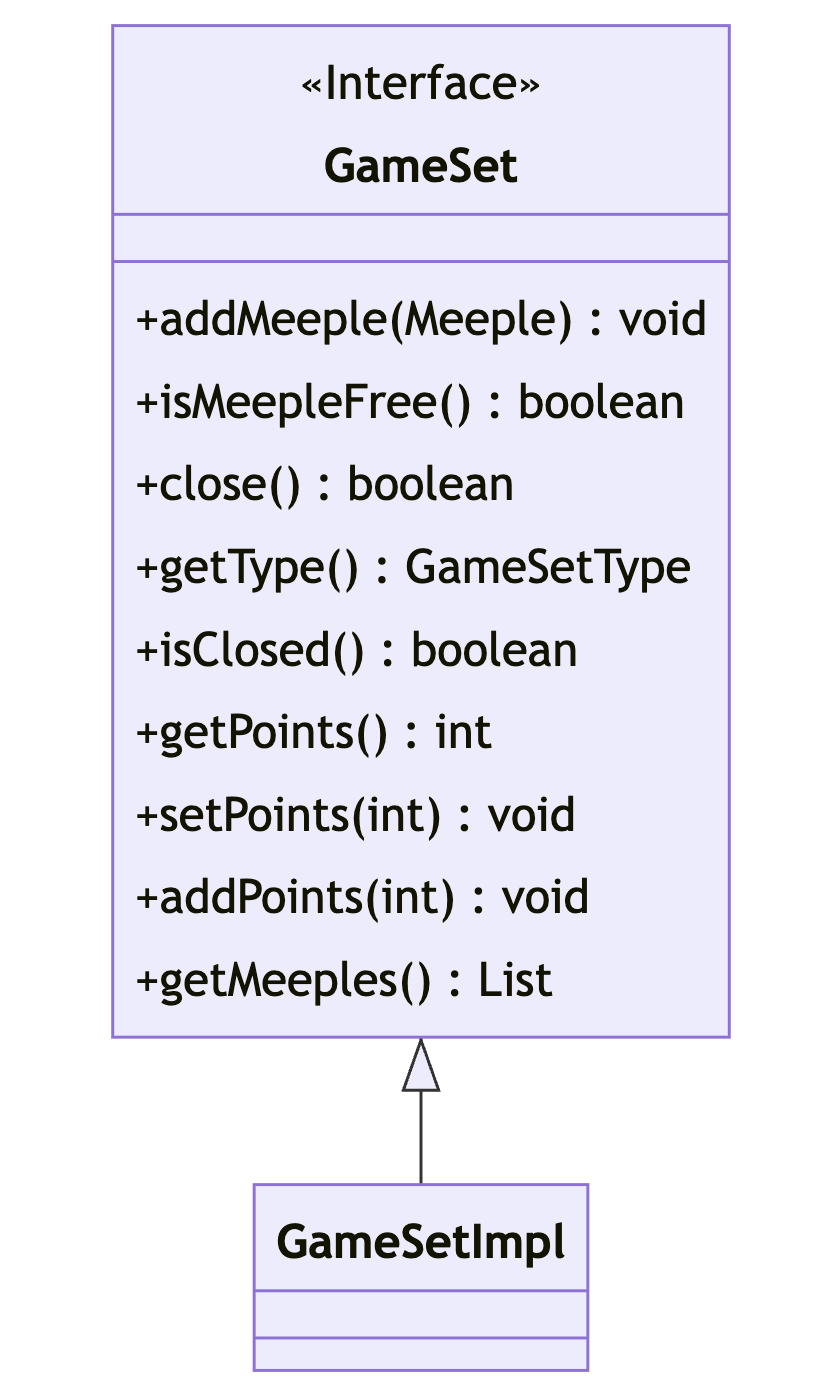
\includegraphics[scale=.4]{images/gameset.png}
    \caption{Rappresentazione UML dell'applicazione del pattern Strategy per il GameSet e GameSetImpl}
\end{figure}
\paragraph{Problema:}
A ogni GameSet, va assegnato il relativo punteggio, il controllo se vi sono meeple presenti e la possibilità di piazzarli, la tipologia del GameSet e infine se è ancora aperto o chiuso.
\paragraph{Soluzione:} 
La classe GameSetImpl implementa lo Strategy pattern, avendo come riferimento GameSet che serve come strategy per la gestione delle informazioni di ogni singolo GameSet.

\subsubsection*{Creazione di più GameSet con tipologie differenti}
\begin{figure}[hh]
    \centering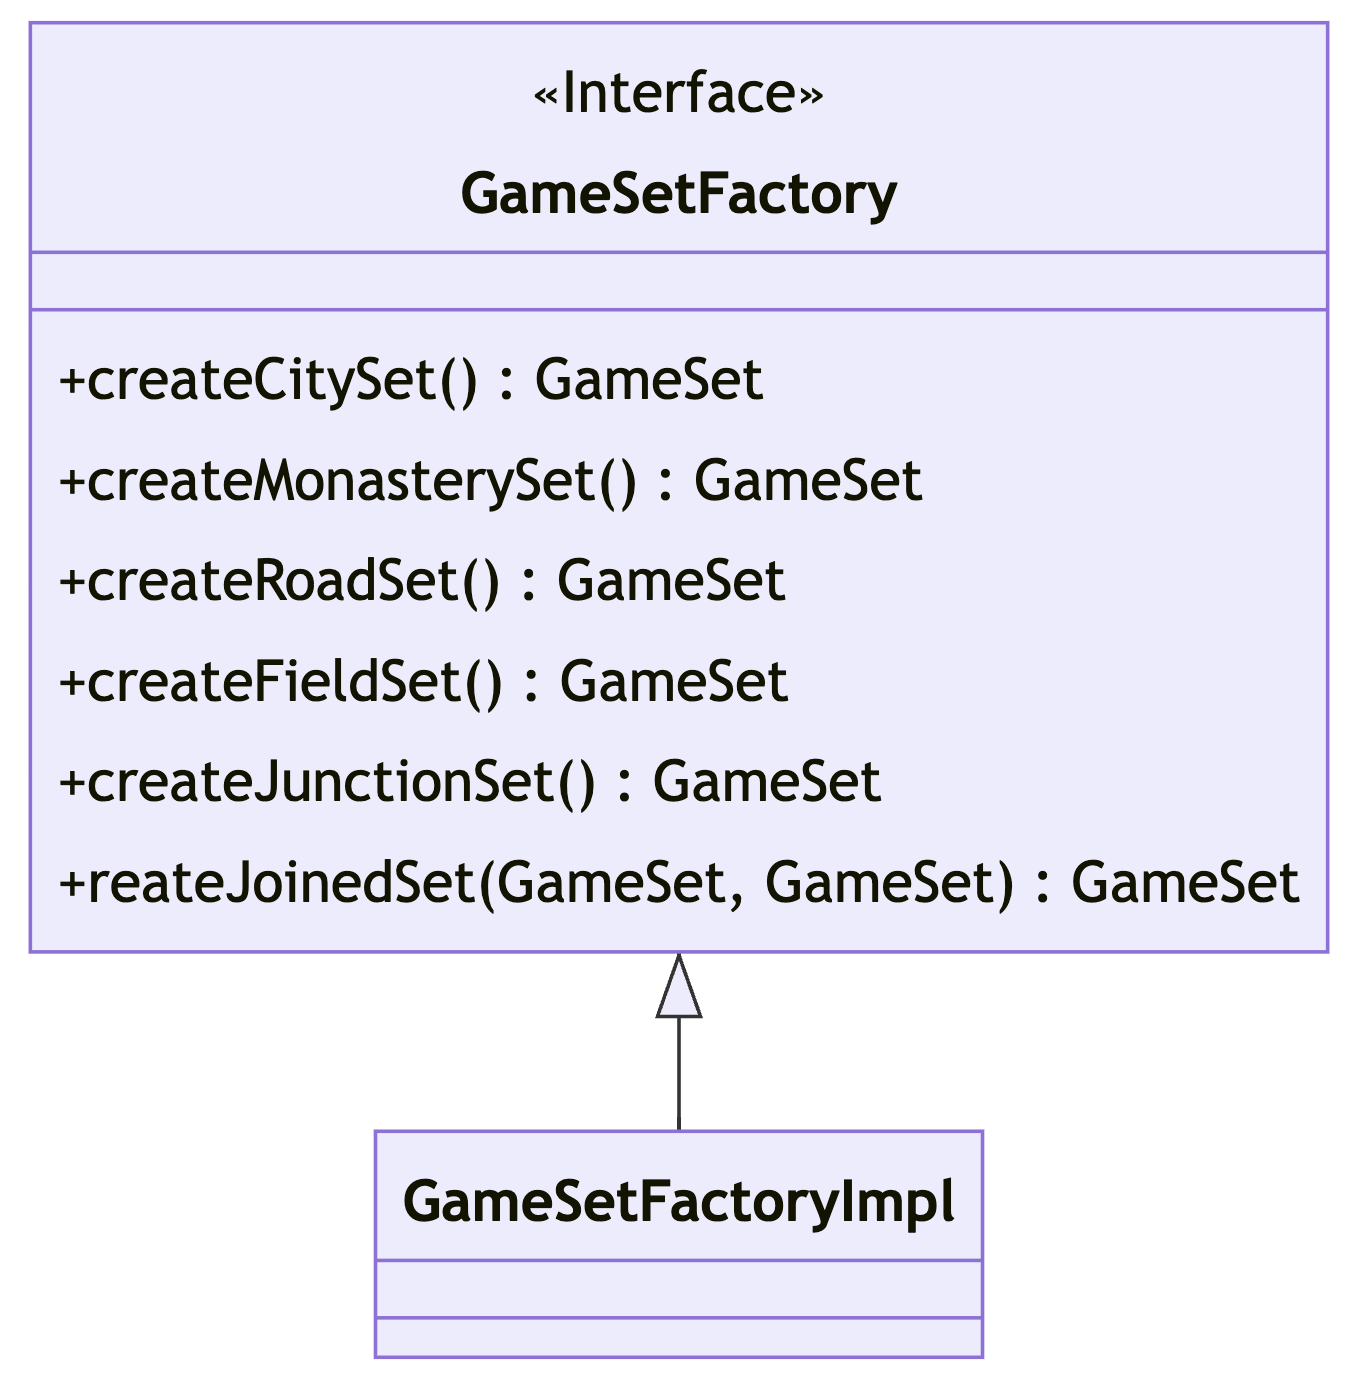
\includegraphics[scale=.3]{images/gamesetfactory.png}
    \caption{Rappresentazione UML dell'applicazione del pattern Strategy per il gamesetfactory e GameSetFactoryImpl}
\end{figure}

\paragraph{Problema:}
Possono esistere più GameSet con informazioni differenti e relativi punteggi assegnati, in aggiunta si devono gestire l'unione di due GameSet.
\paragraph{Soluzione:}
La classe GameSetFactoryImpl implementa lo Strategy pattern, avendo come riferimento GameSetFactory che serve come strategy per la creazione di nuovi GameSet.

\subsection*{Davide Speziali}

\subsection*{Samuele Giancarli}
